% ============================================================================
%  Noise Modelling Hanoi -- handover presentation
%  Build:  latexmk -pdf main.tex        (or: pdflatex main.tex, twice)
%  Notes:  \note{} on every slide. To show them on a second screen, uncomment
%          \setbeameroption{show notes on second screen=right} below.
%
%  Every figure on these slides is traceable to a file in the repository, named
%  on the slide itself. No number is typed by hand: they come from
%  models/metrics.json, models/model_comparison.md and
%  results/tables/hanoi_exceedances.csv.
% ============================================================================
\documentclass[aspectratio=169]{beamer}
\usetheme{metropolis}
\metroset{block=fill, numbering=fraction, progressbar=frametitle}

\usepackage[utf8]{inputenc}
\usepackage[T1]{fontenc}
\usepackage[english]{babel}
\usepackage{booktabs}
\usepackage{graphicx}
\usepackage{xcolor}

% \setbeameroption{show notes on second screen=right}

\definecolor{good}{HTML}{2E7D32}
\definecolor{bad}{HTML}{C62828}
\definecolor{warn}{HTML}{EF6C00}
\newcommand{\src}[1]{{\scriptsize\color{gray}\texttt{#1}}}
\newcommand{\up}[1]{\textcolor{good}{#1}}
\newcommand{\down}[1]{\textcolor{bad}{#1}}

\title{What a smartphone protocol can and cannot establish}
\subtitle{Urban noise in Hanoi --- three months, 363 measurements, three negative results}
\author{Laurian Jamin \and Lucas Zborowski}
\institute{ISIMA, Clermont-Ferrand \\ {}[AFFILIATION TO CONFIRM --- CEI or COSMOS Lab], VinUniversity, Hanoi \\[.4em]
  \scriptsize Supervised by Doanh Nguyen-Ngoc \quad With Nguyen Thanh Quang}
\date{June -- August 2026 \\ \scriptsize Handover meeting}

\begin{document}

\maketitle
\note{Adapt for audience: with the supervisor present, keep the framing short and
go early to the pivot and the negative results. With the incoming team, spend the
time on the last third --- the pipeline, the guards and the handover priorities.

Say up front what the talk is: not a noise map of Hanoi. We cannot produce one and
saying otherwise would be indefensible. It is a methodological study of what this
kind of protocol supports.}

% ---------------------------------------------------------------- 1. why
\section{Why noise in Hanoi}

\begin{frame}{The gap this project sits in}
  \begin{columns}[T]
    \begin{column}{0.55\textwidth}
      \begin{itemize}
        \item Dense, \textbf{motorcycle-dominated} traffic
        \item \textbf{No national strategic noise mapping programme}, no statutory
              noise action plan in Vietnam \\ \src{Nguyen et al. 2025, City Env.\ Interactions}
        \item \textbf{One} instrumented campaign ever published for Hanoi ---
              and it measured in \textbf{2005--2007} \\ \src{Phan et al. 2010, Applied Acoustics}
        \item Class 1 meters and commercial models: out of reach for most local
              research budgets
      \end{itemize}
    \end{column}
    \begin{column}{0.45\textwidth}
      \begin{alertblock}{The question}
        How far does a protocol built from \textbf{three consumer smartphones}
        and \textbf{open data} actually get you?
      \end{alertblock}
    \end{column}
  \end{columns}
\end{frame}
\note{Both citations are verified DOIs --- see docs/literature-review.md. Do not
improvise a health-burden figure here: we did not verify one, and the talk's whole
credibility rests on not inventing numbers.

The twenty-year-old campaign is not a rhetorical flourish. It is the single anchor
of our absolute-bias interval, and its age is why that interval is wide.}

% ---------------------------------------------------------------- 2. questions
\begin{frame}{Research questions --- and what is out of scope}
  \begin{enumerate}
    \item Can OSM morphology predict measured noise at an \textbf{unmeasured location}?
    \item Does a model trained in one city \textbf{transfer} to another?
    \item Does vehicle \textbf{flow from video} explain measured levels?
    \item What can a protocol claim with \textbf{no absolute reference}?
  \end{enumerate}
  \vfill
  \begin{block}{Out of scope --- stated, not discovered later}
    Night-time noise (10 measurements after 21:00, none 00:00--05:00) \quad$\cdot$\quad
    compliance assessment against any standard \quad$\cdot$\quad
    any prediction beyond the three measured sites
  \end{block}
\end{frame}
\note{Declaring the out-of-scope list early is a deliberate move: every one of
these three was a temptation during the project, and two of them were briefly
crossed before being retracted. Saying so at the start buys credibility for the
results later.}

% ---------------------------------------------------------------- 3. state of art
\begin{frame}{State of the art --- ten references, selected by use}
  \begin{columns}[T]
    \begin{column}{0.5\textwidth}
      \textbf{What we lean on}
      \begin{itemize}\small
        \item \textbf{Roberts et al.\ 2017}, \emph{Ecography} --- a CV block must
              exceed the autocorrelation range of the predictors
        \item \textbf{Meyer \& Pebesma 2021}, \emph{MEE} --- area of applicability
        \item \textbf{Kardous \& Shaw 2014}, \emph{JASA} --- smartphones depart from
              reference instruments by several dB, non-constant
        \item \textbf{Phan et al.\ 2010} --- the Hanoi anchor
      \end{itemize}
    \end{column}
    \begin{column}{0.5\textwidth}
      \textbf{Source policy, applied}
      \begin{itemize}\small
        \item \up{\texttt{verified}} --- read in the source (12)
        \item \textcolor{warn}{\texttt{to\_check}} --- second-hand, flagged (2)
        \item \down{\texttt{grey}} --- press-reported, undocumented protocol
              \textbf{never a primary reference} (1)
      \end{itemize}
      \vspace{.6em}
      \begin{exampleblock}{The test of a reliability policy}
        The \textbf{most convenient} figures we had --- twelve Hanoi arteries,
        via the press --- are the ones classified \texttt{grey} and excluded.
      \end{exampleblock}
    \end{column}
  \end{columns}
\end{frame}
\note{If asked why so few references: the criterion was actual use. Each entry says
which decision it informed. Four more are filed as "read, not used, reason".

Quartiles are deliberately blank: Scimago blocks automated access, and quoting a
quartile from a search summary would be second-hand --- exactly what we classify
grey. Fifteen-minute manual task, in the handover.}

% ---------------------------------------------------------------- 4. data
\section{Data}

\begin{frame}{What we collected, and what we publish}
  \small
  \begin{tabular}{@{}llll@{}}
    \toprule
    \textbf{Dataset} & \textbf{Size} & \textbf{Published} & \textbf{Licence} \\
    \midrule
    Field measurements & 363 points, 3 sites & \up{yes} & CC-BY-4.0 \\
    Vehicle counts from video & 147 videos & \up{yes} & CC-BY-4.0 \\
    Survey forms (XLSForm) & 2 forms & \up{yes} & CC-BY-4.0 \\
    Traffic videos & 147, 6.0\,GB & \down{no} & not distributed \\
    Raw Kobo exports & --- & \down{no} & not distributed \\
    OpenStreetMap extract & 49\,146 buildings & \down{no} & ODbL \\
    \bottomrule
  \end{tabular}
  \vfill
  \begin{alertblock}{Ethics --- stated factually}
    \textbf{No institutional ethics review was requested} for the video collection.
    No approval, no exemption, no compliance is claimed. The originals contain faces
    and licence plates and were not anonymised at source; \textbf{only the aggregate
    counts are released}. \\
    \src{docs/data-sources.md --- recommendation: submit to the VinUni ethics committee before any new campaign}
  \end{alertblock}
\end{frame}
\note{Do not soften this slide. A documented limitation is acceptable in a research
record; a compliance claim that was never granted is not, and a reviewer will find it.

If asked about the GPS coordinates: published at full precision. 26 of 363 points
fall inside an OSM building footprint, 13 of them residential --- but none deeper
inside than the worst GPS accuracy of the campaign (7.1 m against 9.0 m), and the
apartment blocks are 26--35 storey towers whose multipath explains the offset.}

% ---------------------------------------------------------------- 5. method
\section{Method}

\begin{frame}{The chain}
  \begin{center}
  \footnotesize
  \begin{tabular}{@{}c@{~$\rightarrow$~}c@{~$\rightarrow$~}c@{~$\rightarrow$~}c@{~$\rightarrow$~}c@{}}
    \textbf{acquisition} & \textbf{preparation} & \textbf{features} & \textbf{selection} & \textbf{map + simulation} \\
    ODK / Kobo & cleaning & OSM 300\,m & 8 models & 40\,m grid \\
    363 points & + weather & morphology & \textbf{3 CV protocols} & 17 hours \\
     & & & \textbf{code picks} & GAMA agents \\
  \end{tabular}
  \end{center}
  \vfill
  \begin{block}{Three protocols, one set of splits}
    \small
    \textbf{Block-CV} 600\,m --- fast, permissive \quad$\cdot$\quad
    \textbf{Buffered LOO} 300\,m --- \emph{the reference: its exclusion radius equals the feature radius} \quad$\cdot$\quad
    \textbf{Leave-one-site-out} --- an unseen typology
  \end{block}
  \src{docs/methodology.md --- 7 assumptions and 3 limitations, each stated where it is made}
\end{frame}
\note{The delivered model is chosen by the code, under the reference protocol,
among candidates fixed before seeing the scores. That guard is the reason the
published map cannot silently inherit a model that only wins a permissive split.

If time is short, this is the slide to compress --- the next two carry the science.}

% ---------------------------------------------------------------- 6. timeline
\begin{frame}{Three months, and one pivot}
  \small
  \begin{tabular}{@{}p{2.4cm}p{10.5cm}@{}}
    \toprule
    \textbf{June} & Reproduce the Uganda dataset; plan: pretrain there, transfer to Hanoi, calibrate locally \\
    \textbf{June--July} & Field campaign: 363 measurements, 3 typologies, 147 videos \\
    \textbf{July} & First model, \down{R\textsuperscript{2} = 0.45 announced}, GAMA simulation built \\
    \midrule
    \textbf{5 August} & \textbf{Internal audit $\rightarrow$ pivot.} No sound level meter would become
                        available; the campaign closed. The project stopped trying to produce a reference
                        noise map --- \emph{it cannot} --- and became a methodological study \\
    \textbf{5--6 August} & Honest CV, baselines, ablation. \down{R\textsuperscript{2} = 0.45 withdrawn:}
                        the split was grouped on 110\,m cells against a 300\,m feature radius \\
    \textbf{11--12 August} & Restructuring for publication and handover \\
    \bottomrule
  \end{tabular}
\end{frame}
\note{The pivot is the honest centre of the story. The audit was ours, written by
us, and it is kept in the repository unchanged --- including the figures it cites
that are now retracted, because an audit whose numbers are corrected afterwards
documents nothing.

Expect the question "why did nobody catch the 0.45 earlier?" Answer: because
reading the code looked fine. That is the next-but-two slide.}

% ---------------------------------------------------------------- 7. results
\section{Results}

\begin{frame}{The ranking inverts --- and that is the result}
  \small
  \begin{tabular}{@{}lccc@{}}
    \toprule
    \textbf{Model} & \textbf{Block-CV 600\,m} & \textbf{Buffered LOO} & \textbf{Leave-one-site-out} \\
                   & \scriptsize permissive & \scriptsize \textbf{reference} & \scriptsize unseen typology \\
    \midrule
    Site $\times$ hour table          & $-0.008$ & $-0.419$ & $-0.058$ \\
    log(dist\_road), 2 param.         & $0.221$ & $0.200$ & $0.189$ \\
    \textbf{Physical kernel, 3 param.} & $0.255$ & \up{$\mathbf{0.246}$} & \up{$\mathbf{0.222}$} \\
    LightGBM v1 (6 features)          & $0.304$ & $0.137$ & $0.029$ \\
    LightGBM v2 (8 features)          & $0.332$ & $0.099$ & $-0.035$ \\
    Hybrid (physics + ML residual)    & \textbf{0.395} & \down{$0.123$} & \down{$0.035$} \\
    \bottomrule
  \end{tabular}
  \vfill
  \begin{alertblock}{}
    The models that win the permissive split are the ones that lose the strict
    splits, \textbf{monotonically}. That is the signature of a model learning the
    sample's spatial autocorrelation, not physics.
  \end{alertblock}
  \src{models/model\_comparison.md --- 95\% CI by block bootstrap, n = 363, 17 blocks}
\end{frame}
\note{This is the scientific core. Do not rush it.

The hybrid is the architecture we recommended ourselves, in writing, in an earlier
draft. We built it, tested it, and it is rejected at this sample size --- not
deferred to future work. Say that explicitly: it is the strongest thing on the slide.

Roberts et al. 2017 predicts exactly this signature. Our finding is a confirmation,
not a discovery --- which is what makes it defensible rather than embarrassing.}

\begin{frame}{The bias--variance trade-off, in numbers}
  \begin{columns}[T]
    \begin{column}{0.5\textwidth}
      \begin{block}{In-sample fit \emph{(worse)}}
        \begin{tabular}{@{}lr@{}}
          R\textsuperscript{2} & $0.499 \rightarrow$ \down{$0.166$} \\
          MAE & $3.79 \rightarrow$ \down{$5.30$ dB} \\
          within $\pm$5 dB & $72.8 \rightarrow$ \down{$53.1\%$} \\
          $\sigma$ simulated & $5.57 \rightarrow$ \down{$3.14$ dB} \\
        \end{tabular}
      \end{block}
    \end{column}
    \begin{column}{0.5\textwidth}
      \begin{block}{Generalisation \emph{(better)}}
        \begin{tabular}{@{}lr@{}}
          Buffered LOO & $0.137 \rightarrow$ \up{$0.246$} \\
          Leave-one-site-out & $0.029 \rightarrow$ \up{$0.222$} \\
        \end{tabular}
      \end{block}
      \vspace{.5em}
      {\small The three-parameter kernel fits the training points \emph{less}
      closely and predicts unmeasured places \emph{better}. The map is flatter
      because the model is less flexible.}
    \end{column}
  \end{columns}
  \vfill
  \src{docs/methodology.md §5.3 --- MAE 5.30 dB read without this slide looks like a bad model}
\end{frame}
\note{This is the slide that makes MAE 5.30 dB defensible. Without the right-hand
column it looks like a regression; with it, it is a documented methodological choice.

The left column is the old LightGBM grid, the right the delivered physical kernel.
Same measurements, same validation code.}

\begin{frame}{The delivered model, and the map}
  \begin{columns}[T]
    \begin{column}{0.52\textwidth}
      \[ E = \frac{A_{hw}}{\max(d_{hw}, D_0)} + \frac{A_{res}}{\max(d_{res}, D_0)} + B \]
      \[ L = 10 \log_{10} E \]
      {\small A line-source attenuation law: energy falls as $1/d$ from two road
      classes, plus a background term. \textbf{Three parameters}, fitted on 363
      points, all constrained non-negative.}
      \vspace{.5em}
      {\footnotesize The learned residual is computed at every run and
      \textbf{deliberately not applied}: under the reference protocol it degrades
      the prediction.}
    \end{column}
    \begin{column}{0.48\textwidth}
      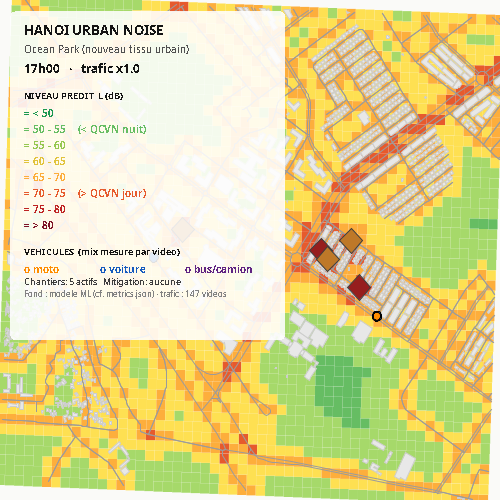
\includegraphics[width=\linewidth]{../results/figures/noise-map-oceanpark-17h.png}
      \src{Ocean Park, 17:00. 40 m grid, 5\,587 cells over 3 sites + 400 m, 17 hours.}
    \end{column}
  \end{columns}
\end{frame}
\note{Point out that the map covers the sampled envelope and nothing more. A grid
was once published over Bach Khoa, a district with zero measurements; it was
retracted and a test now fails if it recurs.

The figure is regenerated by GAMA headless. Its legend cites metrics.json rather
than a hardcoded score --- the previous version of this image displayed the
withdrawn 0.45.}

% ---------------------------------------------------------------- 8. the finding
\section{What the restructuring found}

\begin{frame}{We found one of our own published results was wrong}
  \begin{block}{How}
    Translating figure labels. Re-running the script produced \textbf{a different
    file}.
  \end{block}
  \vspace{.3em}
  The published validation validated \textbf{a grid that no longer existed}:
  regenerated on 5 August when the physical kernel replaced the hybrid, while the
  validation was last built six days earlier. \textbf{Nothing expressed that
  dependency.}
  \vspace{.4em}
  \begin{columns}[T]
    \begin{column}{0.5\textwidth}
      \small \textbf{Published (wrong)} \\
      MAE 3.79 dB, r 0.715, 72.8\% within $\pm$5 dB
    \end{column}
    \begin{column}{0.5\textwidth}
      \small \textbf{Correct} \\
      MAE 5.30 dB, r 0.444, 53.1\% within $\pm$5 dB
    \end{column}
  \end{columns}
  \vspace{.4em}
  \begin{alertblock}{}
    The old figures were \textbf{more flattering} and wrong. Published with the
    trade-off explanation; the old ones archived with their reason; the Makefile now
    carries the dependency so \texttt{make} rebuilds what is stale.
  \end{alertblock}
\end{frame}
\note{Lead with this if the audience is the supervisor. A team that finds its own
result wrong, publishes the worse number and fixes the mechanism is more credible
than a team whose everything works.

A date comparison across the whole tree then found three more stale artefacts, and
two more a level above --- the report and the dashboard, which `make results` did
not rebuild.}

\begin{frame}{Verify by executing, not by reading}
  Every defect this project shipped was one that \textbf{reading could not catch}.
  \vspace{.4em}
  \small
  \begin{tabular}{@{}p{5.2cm}p{8.3cm}@{}}
    \toprule
    \textbf{Guard (it runs)} & \textbf{What it catches} \\
    \midrule
    \texttt{test\_cv\_protocols} & the 110\,m vs 300\,m leak behind R\textsuperscript{2}=0.45 \\
    \texttt{test\_grid\_extent} & a map extended to unmeasured ground \\
    \texttt{test\_features\_extraction} & drift in the input to every published number \\
    \texttt{test\_gama\_fingerprint} & compares \emph{values}, never strings \\
    \texttt{test\_pipeline\_end\_to\_end} & a broken import, \emph{including inside a function} \\
    Makefile dependencies & a derived artefact older than its input \\
    \texttt{make} environment check & an obscure \texttt{ModuleNotFoundError} \\
    \bottomrule
  \end{tabular}
  \vspace{.3em}
  \src{34 tests. Two habits: fingerprint before changing anything; compare commit dates across the whole tree.}
\end{frame}
\note{The renamed-import defect got through three times, twice past reviews that
inspected module headers only --- the third occurrence was inside main(). That is
why the guard executes rather than reads.

This is the slide the incoming team should photograph.}

\begin{frame}{Ten reasoning gaps, moved from code into documentation}
  Each was written only in a comment, where a reviewer would not look.
  \vspace{.5em}
  \begin{itemize}
    \item \textbf{The kernel is fitted in dB, not in energy.} Levels span 47--88 dB
          --- four orders of magnitude in energy --- so a least-squares fit in energy
          would be driven by the loudest points alone. \emph{A choice of loss function
          that determines the published coefficients.}
    \item \textbf{The construction source is calibrated on medians.} Means gave
          74.7 dB, i.e.\ $+8$ dB simulated near a site, against $+2$ dB observed.
    \item \textbf{The exported fleet shares are shares of \emph{density}, not of
          flow.} In congestion density is maximal while flow collapses.
  \end{itemize}
  \vfill
  \begin{exampleblock}{On the calibration}
    A choice made not by preferring the statistic that behaves better, but by
    \textbf{rejecting the one whose output contradicts a field observation}.
  \end{exampleblock}
\end{frame}
\note{Read the closing quote aloud. It is the single sentence that explains why the
calibration is not arbitrary, and it generalises well beyond this project.

Reasoning went into the documentation, a cross-reference stayed in the code, so the
two cannot diverge.}

% ---------------------------------------------------------------- 9. limits
\section{Limits}

\begin{frame}{What we cannot claim}
  \begin{itemize}
    \item \textbf{The instrument is a smartphone application}, not a class 1 or 2
          sound level meter --- the class QCVN 26:2010 requires. This governs the
          uncertainty of every number in this talk.
    \item \textbf{Levels are relative, not absolute.} Three phones cross-calibrated
          against each other, never against a reference. A common bias is invisible
          by construction.
    \item \textbf{The vehicle detector is unvalidated.} Precision, recall and MAPE per
          class unknown; two-wheeler under-detection expected but unquantified.
          \textbf{Modal shares are not publishable.}
    \item \textbf{A 24 s window estimates its hour to roughly $\pm$30\%} (1$\sigma$)
          from sampling alone, measured across 11 site--hour pairs.
    \item \textbf{The night is not sampled.} 10 measurements after 21:00.
    \item \textbf{R\textsuperscript{2} $\approx$ 0.25 is modest} --- and it is the figure that
          survives a split excluding the feature support.
  \end{itemize}
\end{frame}
\note{The 38.6\% QCVN exceedance figure, if asked: it is a descriptive statistic of
our sample, not a finding of non-compliance --- our quantity and our sensors are not
those the standard prescribes. Always say the second half of that sentence.

Never quote the WHO 53/45 values except to say they were withdrawn: they are annual
L_den/L_night averages, not comparable to a 25 s sample.}

% ---------------------------------------------------------------- 10. handover
\section{Handover}

\begin{frame}{Where to start, ranked}
  \begin{enumerate}
    \item \textbf{Validate the detector} --- manual count on 10 videos, about one day.
          \emph{Highest value per effort in the project}: it turns an open-ended
          limitation into a quantified uncertainty, and it is the input uncertainty of
          every downstream number.
    \item \textbf{Extract \texttt{validation.py} and \texttt{physics.py}} from the
          598-line evaluation script --- the most valuable code is the least testable.
    \item \textbf{A real propagation kernel: CNOSSOS-EU via NoiseModelling.}
          \emph{Indicated by our own result}: if a two-parameter distance term beats a
          six-variable learned model, physics corrected by a local residual is the
          architecture the data points at.
  \end{enumerate}
  \vfill
  \begin{block}{Open items --- placeholders, not guesses}
    Affiliation (CEI or COSMOS Lab) $\cdot$ one ORCID $\cdot$ a supervisor title $\cdot$
    a co-authorship decision $\cdot$ \textbf{video retention: custodian, location, deletion deadline}
  \end{block}
\end{frame}
\note{The video retention item is the one with real consequences: 6 GB of
unanonymised footage with faces and plates, currently with no named owner and no
expiry.

If the incoming team is in the room, hand them docs/handover.md and stop there ---
it opens with the working principle, then the open items, then this list.}

\begin{frame}[standout]
  The repository is the deliverable.\\[.6em]
  \normalsize
  \texttt{github.com/Colauz/noise-modelling-hanoi}\\[.8em]
  \small
  \texttt{make setup \&\& make features \&\& make models \&\& make results}\\[.4em]
  {\footnotesize Reproduces the maps and the model comparison from the two datasets
  that ship with it --- no raw Kobo export, no 6 GB of video.}
\end{frame}
\note{Close on this rather than on a summary slide. The claim is checkable in the
room: clone, four commands, same figures.

Questions to expect: why R2 is low (answer with the bias-variance slide); whether
the exceedance rate means non-compliance (no --- descriptive statistic); and what
happens to the videos (open item, supervisor decision).}

\end{document}
